\subsection{UC10 - Visualizzazione Ore Consuntivate }
\begin{itemize}
	\item \textbf{Identificativo}: UC10
	\item \textbf{Nome}: Visualizzazione Ore Consuntivate
	\item\textbf{Descrizione Grafica}: 
	\begin{figure}[h]
		\centering
		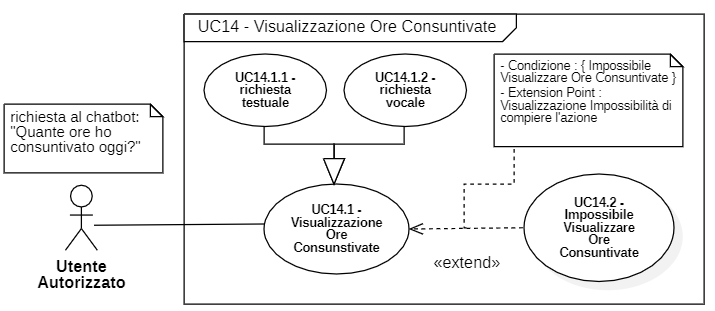
\includegraphics[scale=0.60]{images/UC10.png} 
		\caption{Descrizione grafica caso d'uso UC10}
	 \end{figure}

	\item \textbf{Attori}
	\begin{itemize} 
		\item \textit{Primari}: Utente autorizzato
		\item \textit{Secondari}: Non presenti
	\end{itemize}
	\item \textbf{Descrizione}: l'utente richiede di visualizzare le ore consuntivate; vengono restituite e mostrate tramite chatbot.
	\item \textbf{Precondizione}: Utente ha effettuato il login e si trova nella chat.
	\item \textbf{Postcondizione}: Chatbot restituisce la lista delle Ore consuntivate
	\item \textbf{Scenario principale}:  
		\begin{enumerate}
			\item Utente invia un messaggio al chatbot : "Quante ore ho consuntivato oggi?";
			\item Chatbot restituisce la lista delle Ore consuntivate, con eventuali informazioni.
		\end{enumerate}
\end{itemize}

\subsubsection{UC10.1 Visualizzazione ore consuntivate}
\begin{itemize}
	\item \textbf{Identificativo}: UC10.1
	\item \textbf{Nome}: Visualizzazione ore consuntivate
	\item \textbf{Descrizione Grafica}: (Approfondita in UC10)
	\item \textbf{Attori}
	\begin{itemize}
		\item \textit{Primari}: Utente autorizzato
		\item \textit{Secondari}: Non presenti
	\end{itemize}
	\item \textbf{Descrizione}: l'utente richiede di visualizzare le ore consuntivate durante la giornata.
	\item \textbf{Precondizione}: l'utente invia la richiesta di visualizzazione delle ore consuntivate.
	\item \textbf{Postcondizione}: il chatbot risponde con un messaggio che contiene le ore consuntivate dall'utente.
	\item \textbf{Scenario principale}: 
	\begin{enumerate}
		\item L'utente invia la richiesta al chatbot;
		\item Il chatbot visualizza le ore consuntivate dall'utente.
	\end{enumerate}
\end{itemize}

\paragraph{UC10.1.1 Richiesta testuale}
\begin{itemize}
	\item \textbf{Identificativo}: UC10.1.1
	\item \textbf{Nome}: Richiesta testuale
	\item \textbf{Descrizione Grafica}: (Approfondita in UC10)
	\item \textbf{Attori}
	\begin{itemize}
		\item \textit{Primari}: Utente autorizzato
		\item \textit{Secondari}: Non presenti
	\end{itemize}
	\item \textbf{Descrizione}: l'utente richiede di visualizzare le ore consuntivate durante la giornata tramite input testuale.
	\item \textbf{Precondizione}: l'utente vuole vedere quante ore ha consuntivato.
	\item \textbf{Postcondizione}: l'utente invia la richiesta in formato testuale.
	\item \textbf{Scenario principale}: 
	\begin{enumerate}
		\item L'utente vuole visualizzare le ore consuntivate;
		\item L'utente inserisce testualmente la richiesta.
	\end{enumerate}
\end{itemize}

\paragraph{UC10.1.2 Richiesta vocale}
\begin{itemize}
	\item \textbf{Identificativo}: UC10.1.2
	\item \textbf{Nome}: Richiesta vocale
	\item \textbf{Descrizione Grafica}: (Approfondita in UC10)
	\item \textbf{Attori}
	\begin{itemize}
		\item \textit{Primari}: Utente autorizzato
		\item \textit{Secondari}: Non presenti
	\end{itemize}
	\item \textbf{Descrizione}: l'utente richiede di visualizzare le ore consuntivate durante la giornata tramite input vocale.
	\item \textbf{Precondizione}: l'utente vuole vedere quante ore ha consuntivato.
	\item \textbf{Postcondizione}: l'utente invia la richiesta in formato vocale.
	\item \textbf{Scenario principale}: 
	\begin{enumerate}
		\item L'utente vuole visualizzare le ore consuntivate;
		\item L'utente inserisce tramite input vocale la richiesta.
	\end{enumerate}
\end{itemize}

\subsubsection{UC10.2 Impossibile visualizzare ore consuntivate}
\begin{itemize}
	\item \textbf{Identificativo}: UC10.2
	\item \textbf{Nome}: Impossibile visualizzare ore consuntivate
	\item \textbf{Descrizione Grafica}: (Approfondita in UC10)
	\item \textbf{Attori}
	\begin{itemize}
		\item \textit{Primari}: Utente autorizzato
		\item \textit{Secondari}: Non presenti
	\end{itemize}
	\item \textbf{Descrizione}: l'utente richiede di visualizzare le ore consuntivate durante la giornata ma viene restituito un messaggio d'errore.
	\item \textbf{Precondizione}: l'utente invia la richiesta di visualizzazione delle ore consuntivate.
	\item \textbf{Postcondizione}: il chatbot risponde con un messaggio d'errore indicando l'impossibilità di effettuare l'operazione.
	\item \textbf{Scenario principale}: L'utente richiede di vedere le ore consuntivate, ma gli viene negato e visualizza un messaggio d'errore.
\end{itemize}
\newpage